\documentclass[ignorenonframetext,aspectratio=169]{beamer}
\setbeamertemplate{caption}[numbered]
\setbeamertemplate{caption label separator}{: }
\setbeamercolor{caption name}{fg=normal text.fg}
\beamertemplatenavigationsymbolsempty
\usepackage{lmodern}
\usepackage{amssymb,amsmath}
\usepackage{ifxetex,ifluatex}
\usepackage{fixltx2e} % provides \textsubscript
\ifnum 0\ifxetex 1\fi\ifluatex 1\fi=0 % if pdftex
  \usepackage[T1]{fontenc}
  \usepackage[utf8]{inputenc}
\else % if luatex or xelatex
  \ifxetex
    \usepackage{mathspec}
  \else
    \usepackage{fontspec}
  \fi
  \defaultfontfeatures{Ligatures=TeX,Scale=MatchLowercase}
\fi
% use upquote if available, for straight quotes in verbatim environments
\IfFileExists{upquote.sty}{\usepackage{upquote}}{}
% use microtype if available
\IfFileExists{microtype.sty}{%
\usepackage{microtype}
\UseMicrotypeSet[protrusion]{basicmath} % disable protrusion for tt fonts
}{}
\newif\ifbibliography
\hypersetup{
            pdfborder={0 0 0},
            breaklinks=true}
\urlstyle{same}  % don't use monospace font for urls

% Prevent slide breaks in the middle of a paragraph:
\widowpenalties 1 10000
\raggedbottom

\AtBeginPart{
  \let\insertpartnumber\relax
  \let\partname\relax
  \frame{\partpage}
}
\AtBeginSection{
  \ifbibliography
  \else
    \let\insertsectionnumber\relax
    \let\sectionname\relax
    \frame{\sectionpage}
  \fi
}
\AtBeginSubsection{
  \let\insertsubsectionnumber\relax
  \let\subsectionname\relax
  \frame{\subsectionpage}
}

\setlength{\parindent}{0pt}
\setlength{\parskip}{6pt plus 2pt minus 1pt}
\setlength{\emergencystretch}{3em}  % prevent overfull lines
\providecommand{\tightlist}{%
  \setlength{\itemsep}{0pt}\setlength{\parskip}{0pt}}
\setcounter{secnumdepth}{0}
\usepackage[default]{lato}
\pdfmapfile{=lato.map}
\usepackage[official]{eurosym}
\usepackage{booktabs}
\usepackage[makeroom]{cancel}
\usepackage{amsmath}
\usepackage{tikz} 

\makeatletter
\newif\if@borderstar
\def\bordermatrix{\@ifnextchar*{%
\@borderstartrue\@bordermatrix@i}{\@borderstarfalse\@bordermatrix@i*}%
}
\def\@bordermatrix@i*{\@ifnextchar[{\@bordermatrix@ii}{\@bordermatrix@ii[()]}}
\def\@bordermatrix@ii[#1]#2{%
\begingroup
\m@th\@tempdima8.75\p@\setbox\z@\vbox{%
\def\cr{\crcr\noalign{\kern 2\p@\global\let\cr\endline }}%
\ialign {$##$\hfil\kern 2\p@\kern\@tempdima & \thinspace %
\hfil $##$\hfil && \quad\hfil $##$\hfil\crcr\omit\strut %
\hfil\crcr\noalign{\kern -\baselineskip}#2\crcr\omit %
\strut\cr}}%
\setbox\tw@\vbox{\unvcopy\z@\global\setbox\@ne\lastbox}%
\setbox\tw@\hbox{\unhbox\@ne\unskip\global\setbox\@ne\lastbox}%
\setbox\tw@\hbox{%
$\kern\wd\@ne\kern -\@tempdima\left\@firstoftwo#1%
\if@borderstar\kern2pt\else\kern -\wd\@ne\fi%
\global\setbox\@ne\vbox{\box\@ne\if@borderstar\else\kern 2\p@\fi}%
\vcenter{\if@borderstar\else\kern -\ht\@ne\fi%
\unvbox\z@\kern-\if@borderstar2\fi\baselineskip}%
\if@borderstar\kern-2\@tempdima\kern2\p@\else\,\fi\right\@secondoftwo#1 $%
}\null \;\vbox{\kern\ht\@ne\box\tw@}%
\endgroup
}
\makeatother


\graphicspath{{G:/FSD_RestrictedAccess/RESIDENTIAL/FT/720dpd/fs_note/Draft/}}

\newcommand{\chartit}[1]{
\includegraphics{#1}
}


\makeatletter
\def\input@path{{G:/FSD_RestrictedAccess/RESIDENTIAL/FT/720dpd/fs_note/Draft/}}
\makeatother


\setbeamertemplate{itemize subitem}{\scriptsize{{--}}}
\setbeamertemplate{itemize item}{\scriptsize{$\bullet$}}

\title{Gambling On A Recovery:\\
Firm Leverage, Investment and Cash Holding During Crises}
\author{Monica Petrescu\\[2\baselineskip]Discussion by\\
Terry O'Malley\\
(University College Dublin)}
\date{06 September, 2018}

\begin{document}
\frame{\titlepage}

\begin{frame}{Overview}

\begin{itemize}
\item
  Excess cash holding by firms usually attributed to insurance motive
\item
  In a recession, there is a type of carry trade available: a
  \emph{gambling motive}
\item
  Borrow long in a recession at low interest ratesto benefit if the
  upturn arrives soon
\end{itemize}

\end{frame}

\begin{frame}{Intuition}

\begin{itemize}
\item
  Borrowing in a recession at low rates has positive \emph{option value}
\item
  Think of it like purchasing a call option on a stock

  \begin{itemize}
  \tightlist
  \item
    Your downside is capped because of limited liability
  \item
    Might also be more valuable if you can do a carry trade: lend at
    short maturity
  \item
    Your upside is large because you borrow low and have option to
    invest at this low rate if the next period is an economic expansion.
  \end{itemize}
\item
  Call option on future positive states of the world
\end{itemize}

\end{frame}

\begin{frame}{Insurance v gambling}

\begin{itemize}
\tightlist
\item
  If I see companies holding higher amounts of \emph{both} long-term
  debt and cash, can I say it is because of:
\end{itemize}

\begin{enumerate}
\def\labelenumi{\arabic{enumi}.}
\item
  \emph{Insurance policy}. I like to keep cash on hand because then my
  downside is limited when I have low-cash flow.
\item
  \emph{Gambling}. I like to keep cash on hand because then my upside is
  unlimited when the economy picks up.
\end{enumerate}

\begin{itemize}
\tightlist
\item
  Gambling equilibrium can emerge as long as investors receive a premium
  on the risk-free rate and managers cannot divert large amount of cash.
\end{itemize}

\end{frame}

\begin{frame}{Empirical Analysis}

\begin{itemize}
\item
  Compustat panel data, quarterly 1990-2014
\item
  Theoretically, should be a \emph{more positive} reduced-form
  relationship between firm debt and cash holdings at the end of a
  recession
\item
  Data supports this conclusion
\end{itemize}

\end{frame}

\begin{frame}{Discussion}

\begin{itemize}
\item
  Paper is mostly theory
\item
  I am an empiricist
\item
  Final section is empirical and work-in-progress
\end{itemize}

\(\implies\) Everybody gains from a discussion focused on empirical
strategy

\end{frame}

\begin{frame}{Thoughts}

\begin{itemize}
\item
  Do expectations and default costs distinguish gamblers and insurees?
\item
  Does the slope of yield curve affect gambling?
\item
  How likely is gambling to arise if investors have perfect information
  about firm's debt levels?
\end{itemize}

\end{frame}

\begin{frame}{Empirical Strategy}

\begin{itemize}
\tightlist
\item
  \emph{Very} difficult to identify the mechanism in question

  \begin{itemize}
  \tightlist
  \item
    work in progress
  \end{itemize}
\item
  Strategy is to estimate the relationship between \(\Delta\text{Debt}\)
  and \(\Delta\text{Cash}\) and see if it changes during a recession
\end{itemize}

\[\Delta\text{Cash}_{it} = \gamma\Delta\text{Long Term Debt}_{it} + 
\delta\text{Recession}_t + 
\beta\Delta\text{Long Term Debt}_{it} \times \text{Recession}_t + X_{it} + \epsilon_{it}\]

\begin{itemize}
\tightlist
\item
  \(\beta\) should be positive because gambling should be seen during
  this time period
\end{itemize}

\end{frame}

\begin{frame}{Empirical results}

Effect size of recession interaction

\begin{minipage}[c]{0.48\linewidth}
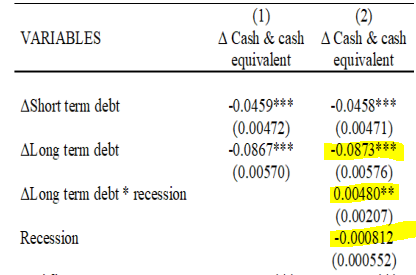
\includegraphics[width=0.8\linewidth]{interact}
\end{minipage}\begin{minipage}[c]{0.48\linewidth}
\begin{itemize}
\item Positive interaction suggesting relationship becomes {\bf less negative}
\item Main effect dominates (not necessarily a problem)
\item Direction is in line with theory but effect is very small \end{itemize}\end{minipage}

\end{frame}

\begin{frame}{Specification}

\begin{itemize}
\item
  Reduced-form seems to capture some gambling but design has some issues
\item
  Pooled OLS: lots of variation behind these estimates, is it the right
  type?
\item
  Only 1 recession

  \begin{itemize}
  \tightlist
  \item
    No fixed effects
  \item
    Inference: need more
  \item
    Regional variation in US recession? Cross-country variation?
  \end{itemize}
\item
  Slope of yield curve
\end{itemize}

\end{frame}

\begin{frame}{Omitted variable bias?}

\begin{itemize}
\item
  Specification relies on between-firm variation
\item
  Potential for OVB

  \begin{itemize}
  \tightlist
  \item
    Lurking confounder causes debt and cash
  \end{itemize}
\item
  Sectoral fixed effects: within-sector variation
\item
  Survival bias: are firms leaving sample due to bankruptcy?
\end{itemize}

\end{frame}

\begin{frame}{Conclusion}

\begin{itemize}
\item
  Very interesting theoretical insight
\item
  But very difficult to test empirically
\end{itemize}

\end{frame}

\end{document}
